	%% The following is a directive for TeXShop to indicate the main file
%%!TEX root = diss.tex

\chapter{Introduction}
\label{ch:Introduction}

\begin{epigraph}
    \emph{If I have seen farther it is by standing on the shoulders of
    Giants.} ---~Sir Isaac Newton (1855)
\end{epigraph}

Computational Fluid Simulations (CFD) is a field of study where scientists and engineers architect new ways to numerically solve fluid flow equations. Before the advent of computers, numerical solutions of differential equations was done by hand. This lead to a great deal of work in the direction of creating faster algorithms to solve differential equations. An example is the development of the Fast Fourier Transform (FFT) by Cornelius Lancoz to increase the computation speed of Discrete Fourier Transform (DFT). However, since the development and advancement of computers, engineers had a significant amount of compute power to work with. This lead to the development of highly accurate methods (as compared to before) to simulate flow over various objects. These simulations have since gotten bigger and better, typically including millions of degrees of freedom, even starting to touch a billion in regular industry use.

\section{Mesh Generation - A brief overview}

The equations which govern the conservation of mass, momentum and energy of a moving fluid also called Navier-Stokes equations are solved in the given domain to simulate fluid flow in that domain. In order to numerically solve these equations, we need a discretization of the given domain. This discrete basis required to solve the Navier-Stokes equations is called a mesh. Simply put, a mesh is a collection of points, lines and cells that together construct the space around a body in a fluid flow.

The process of discretization of the domain to form the basis of solving the Navier-Stokes equations, or any other differential equation numerically is called mesh generation. Save a few exotic methods, almost all of the techniques in CFD require a mesh to solve the flow on. Traditionally, mesh generation was a very manual process, where engineers used to place the mesh points and cells by hand. Such heuristic approach to mesh generation gave them a lot of freedom in discretizing the domain. Cells could be aligned to the boundaries of objects. The quality of the cells, which was taken as some measure of the interior angle of the cells, was almost always chosen to be good. The benefits of this method were quite evident. However, there were some major drawbacks. The process of mesh generation was incredibly slow. Engineers would spend hours, sometime days to create the mesh for a given geometry. Also, mesh adaptation with solution was almost non-existant because that would have made the process even slower.

\begin{definition}
A \textbf{mesh} $M$ is a geometrical discretization of a domain $\Omega$ that consists of (a) a collection of mesh entities $M_i$ of controlled size and distribution and (b) topological relationships or adjacencies forming the graph of the mesh. The mesh $M$ covers $\Omega$ without neither overlap nor hole.
\end{definition}

\begin{figure}
  \centering
  \begin{subfigure}{0.5\linewidth}
    \centering
    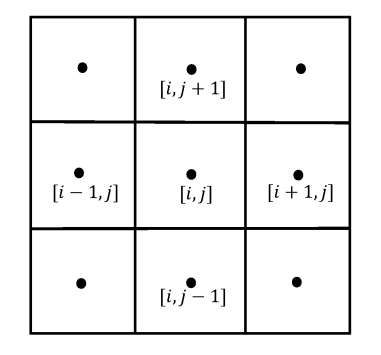
\includegraphics[width=0.8\linewidth]{img/intro/mStructured.png}
    \caption{}
    \label{fig-structured-ij}
  \end{subfigure}%
  \begin{subfigure}{0.5\linewidth}
    \centering
    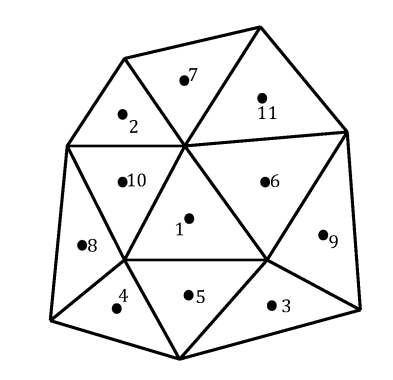
\includegraphics[width=0.8\linewidth]{img/intro/mUnstructured.png}
    \caption{fig-unstructured-ij}
    \label{fig-unstructured}
  \end{subfigure}%
  \caption{}
  \label{fig-structured-unstructured}
\end{figure}

\section{Structured and Unstructured Meshes}

The evolution of mesh generation can be correlated to the evolution of compute power available to the boffins. With the advent of third generation computers (1964-1971) carryinig integrated circuits, engineers were able to automate some of the manual processes in mesh generation. Meshes consisting of a template that repeats itself could be generated. These meshes were called \textit{structured meshes} as their adjacencies or relationships could be known implicitly. Consider a grid in two dimensions as shown in Figure \ref{fig-structured-ij}. Given a cell $(i,j)$ we can identify its neighbours as $(i-1, j)$ to the left and $(i+1, j)$ to the right. Similarly, cell $(i, j+1)$ will be to the top and $(i, j-1)$ would be to its bottom. The connectivity pattern repeats in such a mesh. Figure \ref{fig-structuredNaca0012} shows a structured mesh generated for NACA 0012 airfoil around its leading edge. Notice the implicit connectivity of the cells even though the size of mesh elements is varying.

\begin{figure}
  \centering
  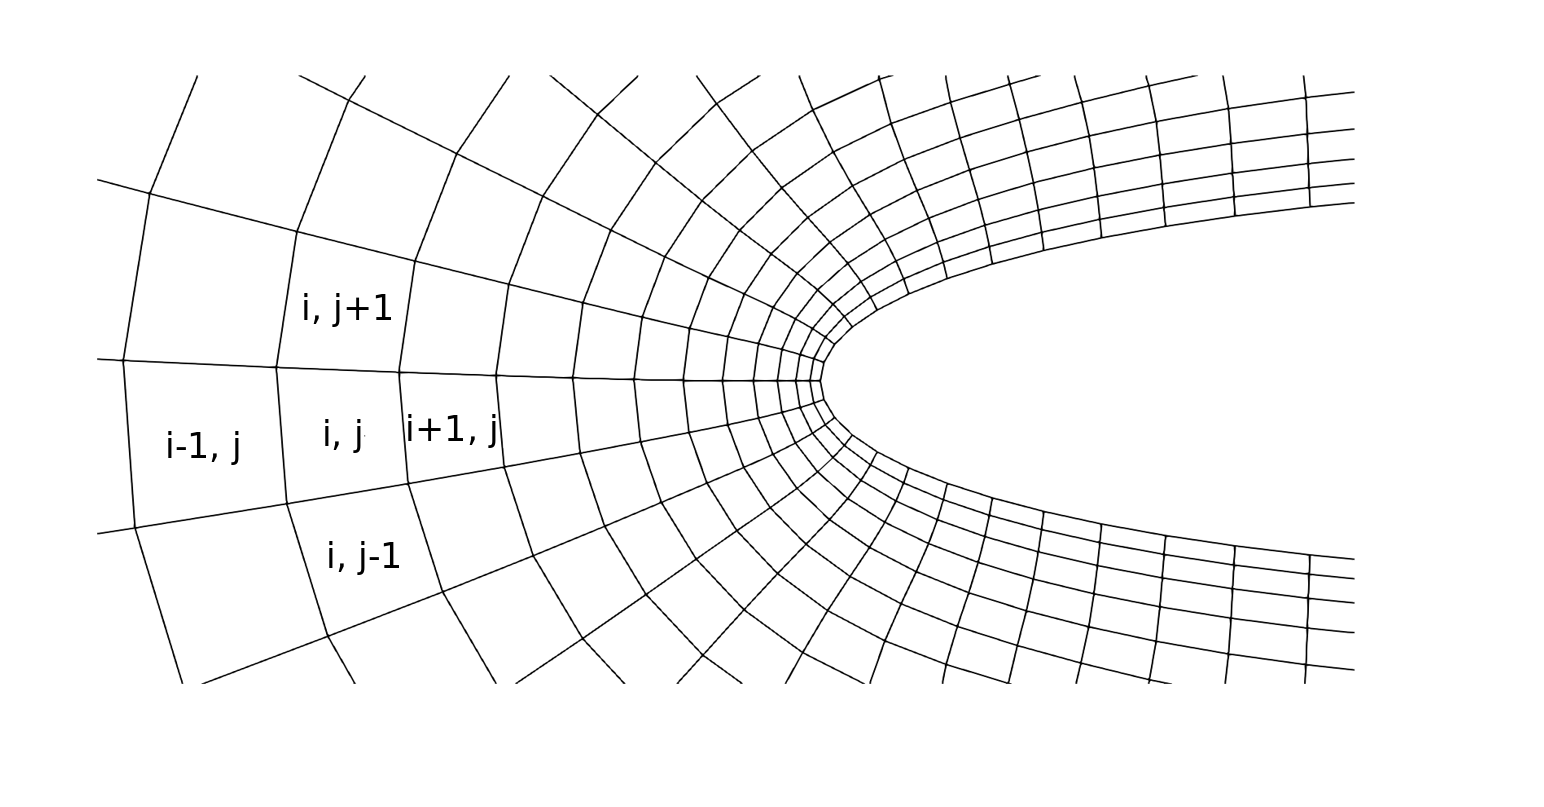
\includegraphics[width=0.8\linewidth]{img/intro/stucturedNaca0012.png}
  \caption{Structured mesh around leading edge of a NACA 0012 airfoil}
  \label{fig-structuredNaca0012}
\end{figure}


Structured meshes were attractive to engineers because of their low memory usage as the topology of the cells is repeated. Also, given simple domains to mesh, these meshes were optimal for minimizing the errors in CFD, resulting in faster simulations \cite{d1991optimal}. Programming CFD solvers with these meshes was easy as cell connectivity occurs in a regular fashion. However, as the scope of CFD simulations grew over time and more complex geometries were becoming commonplace, the task of generating structured meshes around them proved to be a daunting one. 

The disadvantage of using a structured mesh for more complex geometries is the increase in grid non-orthogonality or skewness that can cause unphysical solutions due to the transformation of the governing equations \cite{TU2013219}. The transformed equations that accommodate the non-orthogonality act as the link between the structured coordinate system (such as Cartesian coordinates) and the body-fitted coordinate system, but contain additional terms, thereby augmenting the cost of numerical calculations and difficulties in programming. Hence, a structured mesh may affect the accuracy and the efficiency of the numerical schemes used by a solver. Additionally, the tedious process of generating such meshes for more complex geometries was hard to justify. Hence, more flexible and automatic methods were devised. These methods produced meshes in a more random manner but with lesser human intervention. Broadly, the meshes produced by such methods were classified as \textit{unstructured meshes}. Figure \ref{fig-unstructured} shows an unstructured mesh. The arrangement of the mesh elements is random. Along with the shape of the elements, we need a data structure to store the adjacencies of the mesh.

The cost of finding flux at a wall, a widely used parameter in Finite Volume Methods (FVM), for unstructured meshes is high as compared to their structured counterparts. Also, the amount of memory usage is also high as the topology of the mesh is no longer repeated. Still, they are more widely used today because of their capability to handle arbitrary complex geometries, their capability to automate the mesh generation process and their flexibility in refinement based on the geometry topology and/or the solution gradients. Figure \ref{fig-unstructuredNaca0012} shows an unstructured mesh at the leading edge of a NACA 0012 airfoil. Notice the random arrangement of triangles around the airfoil geometry. The connectivity at each vertex of the mesh needs to be stored separately.

\begin{figure}
  \centering
  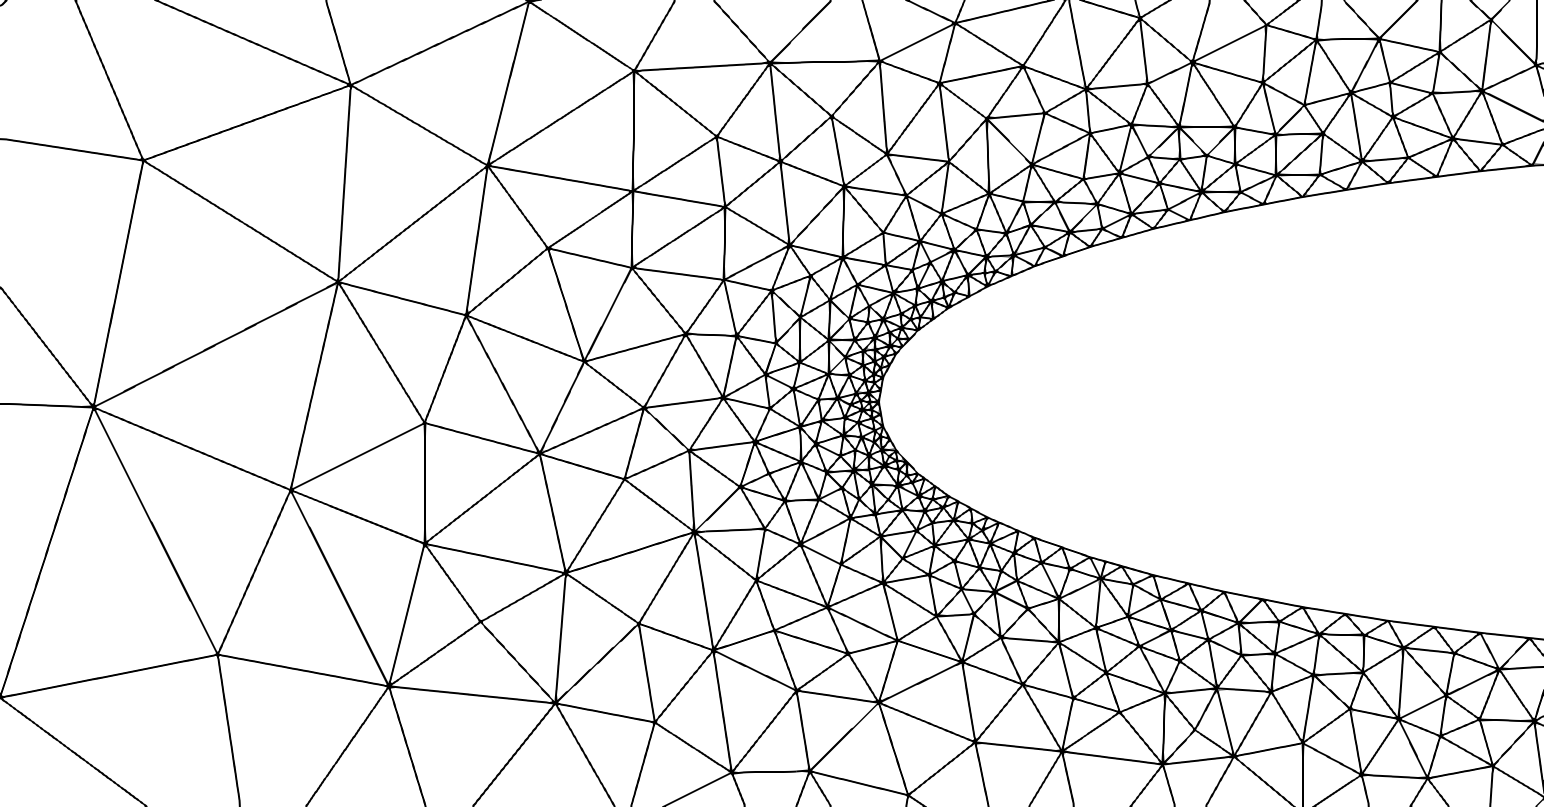
\includegraphics[width=0.8\linewidth]{img/intro/unstructuredNaca0012.png}
  \caption{Unstructured mesh around leading edge of NACA 0012 airfoil}
  \label{fig-unstructuredNaca0012}
\end{figure}

\section{Simplicial and Non-Simplicial Meshes}

Before discussing about simplicial and non-simplicial meshes, we need to define certain terms. In geometry, a simplex is a generalization of teh notion of a triangle or tetrahedron to arbitrary dimensions. For example, a 0-simplex is a point, a 1-simplex is a line segment, a 2-simplex is a triangle and a 3- simplex is a tetrahedron. See Figure \ref{fig-simplices} for an illustration.

\begin{figure}
	\centering
	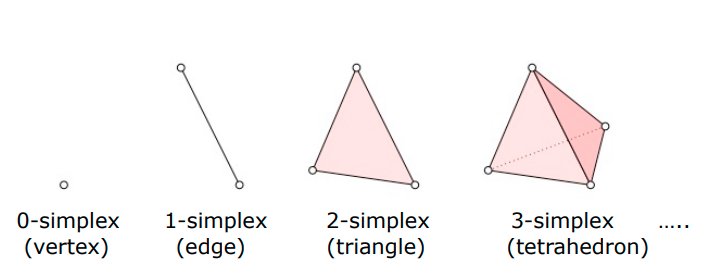
\includegraphics[width=0.95\linewidth]{img/intro/simplices.png}
	\caption{$n$ dimesnional simplices.}
	\label{fig-simplices}
\end{figure}

\begin{definition}
A \textbf{k-simplex} is a k-dimensional polytope which is the convex hull of its k+1 vertices
\end{definition}

A simplicial complex is a set composed of points, line segments, triangles, and their n-dimensional counterparts. In other words, a simplicial complex is a set strictly containing simplices only. Figure \ref{fig-simplicialComplex} shows a three-dimensional simplicial complex.

\begin{definition}
A \textbf{simplicial complex} K
is a set of simplices that
satisfies the two following
conditions:
a) Any face of a simplex
 from K is also in K
b) The intersection of any
 two simplices S1 and S2
 is either $\phi$ (null set) or a face of
 both S1 and S2
\end{definition}

\begin{figure*}
\begin{minipage}{0.45\linewidth}
	\centering
	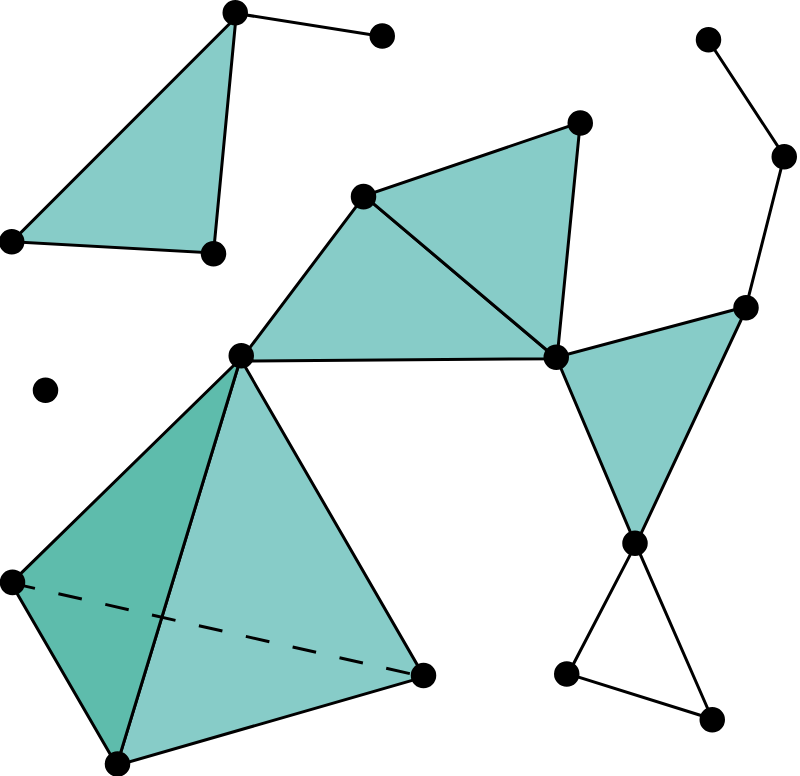
\includegraphics[width=\linewidth]{img/intro/simplicalComplex.png}
	\caption{A three-dimensional simplicial complex.}
	\label{fig-simplicialComplex}
\end{minipage}\hfill
\begin{minipage}{0.45\linewidth}
	\centering
	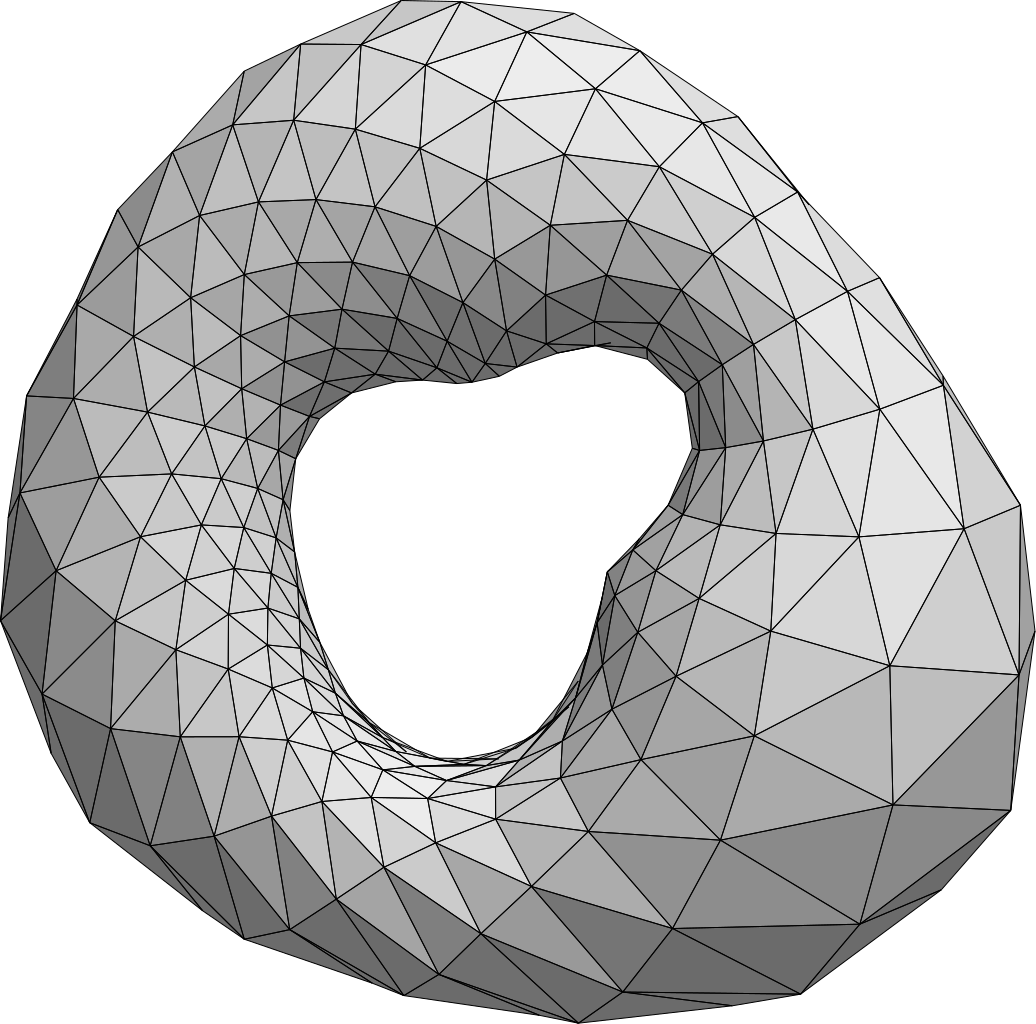
\includegraphics[width=\linewidth]{img/intro/triangulation.png}
	\caption{Triangulation of a torus.}
	\label{fig-triangulation}
\end{minipage}
\end{figure*}

A mesh which contains only simplicial mesh elements is called a simplicial mesh. For example, a mesh which contains only triangular simplices is called a triangulaiton. In other words, a \textbf{triangulation} is the division of a surface or plane polygon into a set of triangles, usually with the restriction that each triangle side is entirely shared by two adjacent triangles. It was proved in 1925 that every surface has a triangulation, but it might require an infinite number of triangles. Figure \ref{fig-triangulation} shows a triangulation of a torus.

\begin{definition}
	A \textbf{triangulation} of a topological space X is a simplicial complex K, homeomorphic to X, together with a homeomorphism h: K $\rightarrow$ X.
\end{definition}

A non-simplicial mesh is simply a mesh which is not simplicial. Such a mesh contains mesh elements other than simplices too. For example, in two dimensions, a mesh which contains quadrilateral elements or quads will be called a non-simplicial mesh. In three dimensions, a mesh containing hexahedral elements would fall under the category of non-simplicial meshes.

Simplicial elements have been traditionally used for mesh generation. These elements are simple to work with and provide good flexibility in terms of discretization of a domain. These benefits make simplicial meshes very simple to produce. However, some of the drawbacks of simplicial meshes have led to mesh generation techniques with non-simplicial elements. Consider a triangulation of a surface. The Euler Formula states that for any convex polyhedron, the number of vertices and faces together is exactly two more than the number of edges. Mathematically,

\begin{equation}
V-E+F=2
\label{eqn-eulerFormula}
\end{equation}

where $V$ is the number of vertices, $E$ is the number of edges and $F$ is the number of faces in the polyhedron. For a triangulation, each edge is shared by two faces. Also, each face has three edges associated with it. Hence, the number of faces is $2/3$ times the number of edges, or $F= (2/3) \times E$. Substituting this in equation \ref{eqn-eulerFormula}, we get

\begin{align}
\begin{split}
		V - E + F  & = 2 \\
		V - E + \frac{2}{3} \: E & = 2 \\
		V - \frac{1}{3} \: E & = 2 \\
		3V & \approx E
		\end{split}
\end{align}

Hence, the number of edges is three times the number of vertices in a triangulation (asymptotically). On the other hand, the number of edges is two times the number of vertices for a closed quadrilateral surface mesh. A similar derivation could be done for three-dimensional simplicial and non-simplicial elements. The number of edges in a tetrahedral mesh is about seven times the number of vertices. On the other hand, in a hexahedral mesh, the number of edges is only about three times the number of vertices (asymptotically). Higher connectivity for simplical meshes leads to higher computational cost when refining the mesh using a vertex-based discretization methods. Hence, non-simplicial meshes are substantially more efficient than simplical meshes for a given number of unknowns or grid points.

Additionally, regular arrays of nonsimplical elements may also enhance accuracy, owing to a local cancellation of truncation errors that may not occur on groups of nonsimilar simplical elements \cite{mavriplis1997unstructured}. In two-dimensions, quadrilateral elements have been preferred over triangles in highly stretched two-dimensional grids due to their lower connectivity \cite{aftosmis1994accuracy}. These advantages of non-simplical mesh elements have resulted in fully non-simplicial mesh generation techniques \cite{blacker1991paving, zhu1991new}. The scheme introduced by Blacker \etal uses a paving methodology with several mesh element collision checks and special conditions for the concave corners to generated an isotropic all-quad two-dimensional mesh for complex geometries. One such mesh is shown in Figure \ref{fig-quadMesh}.

\begin{figure}
	\centering
	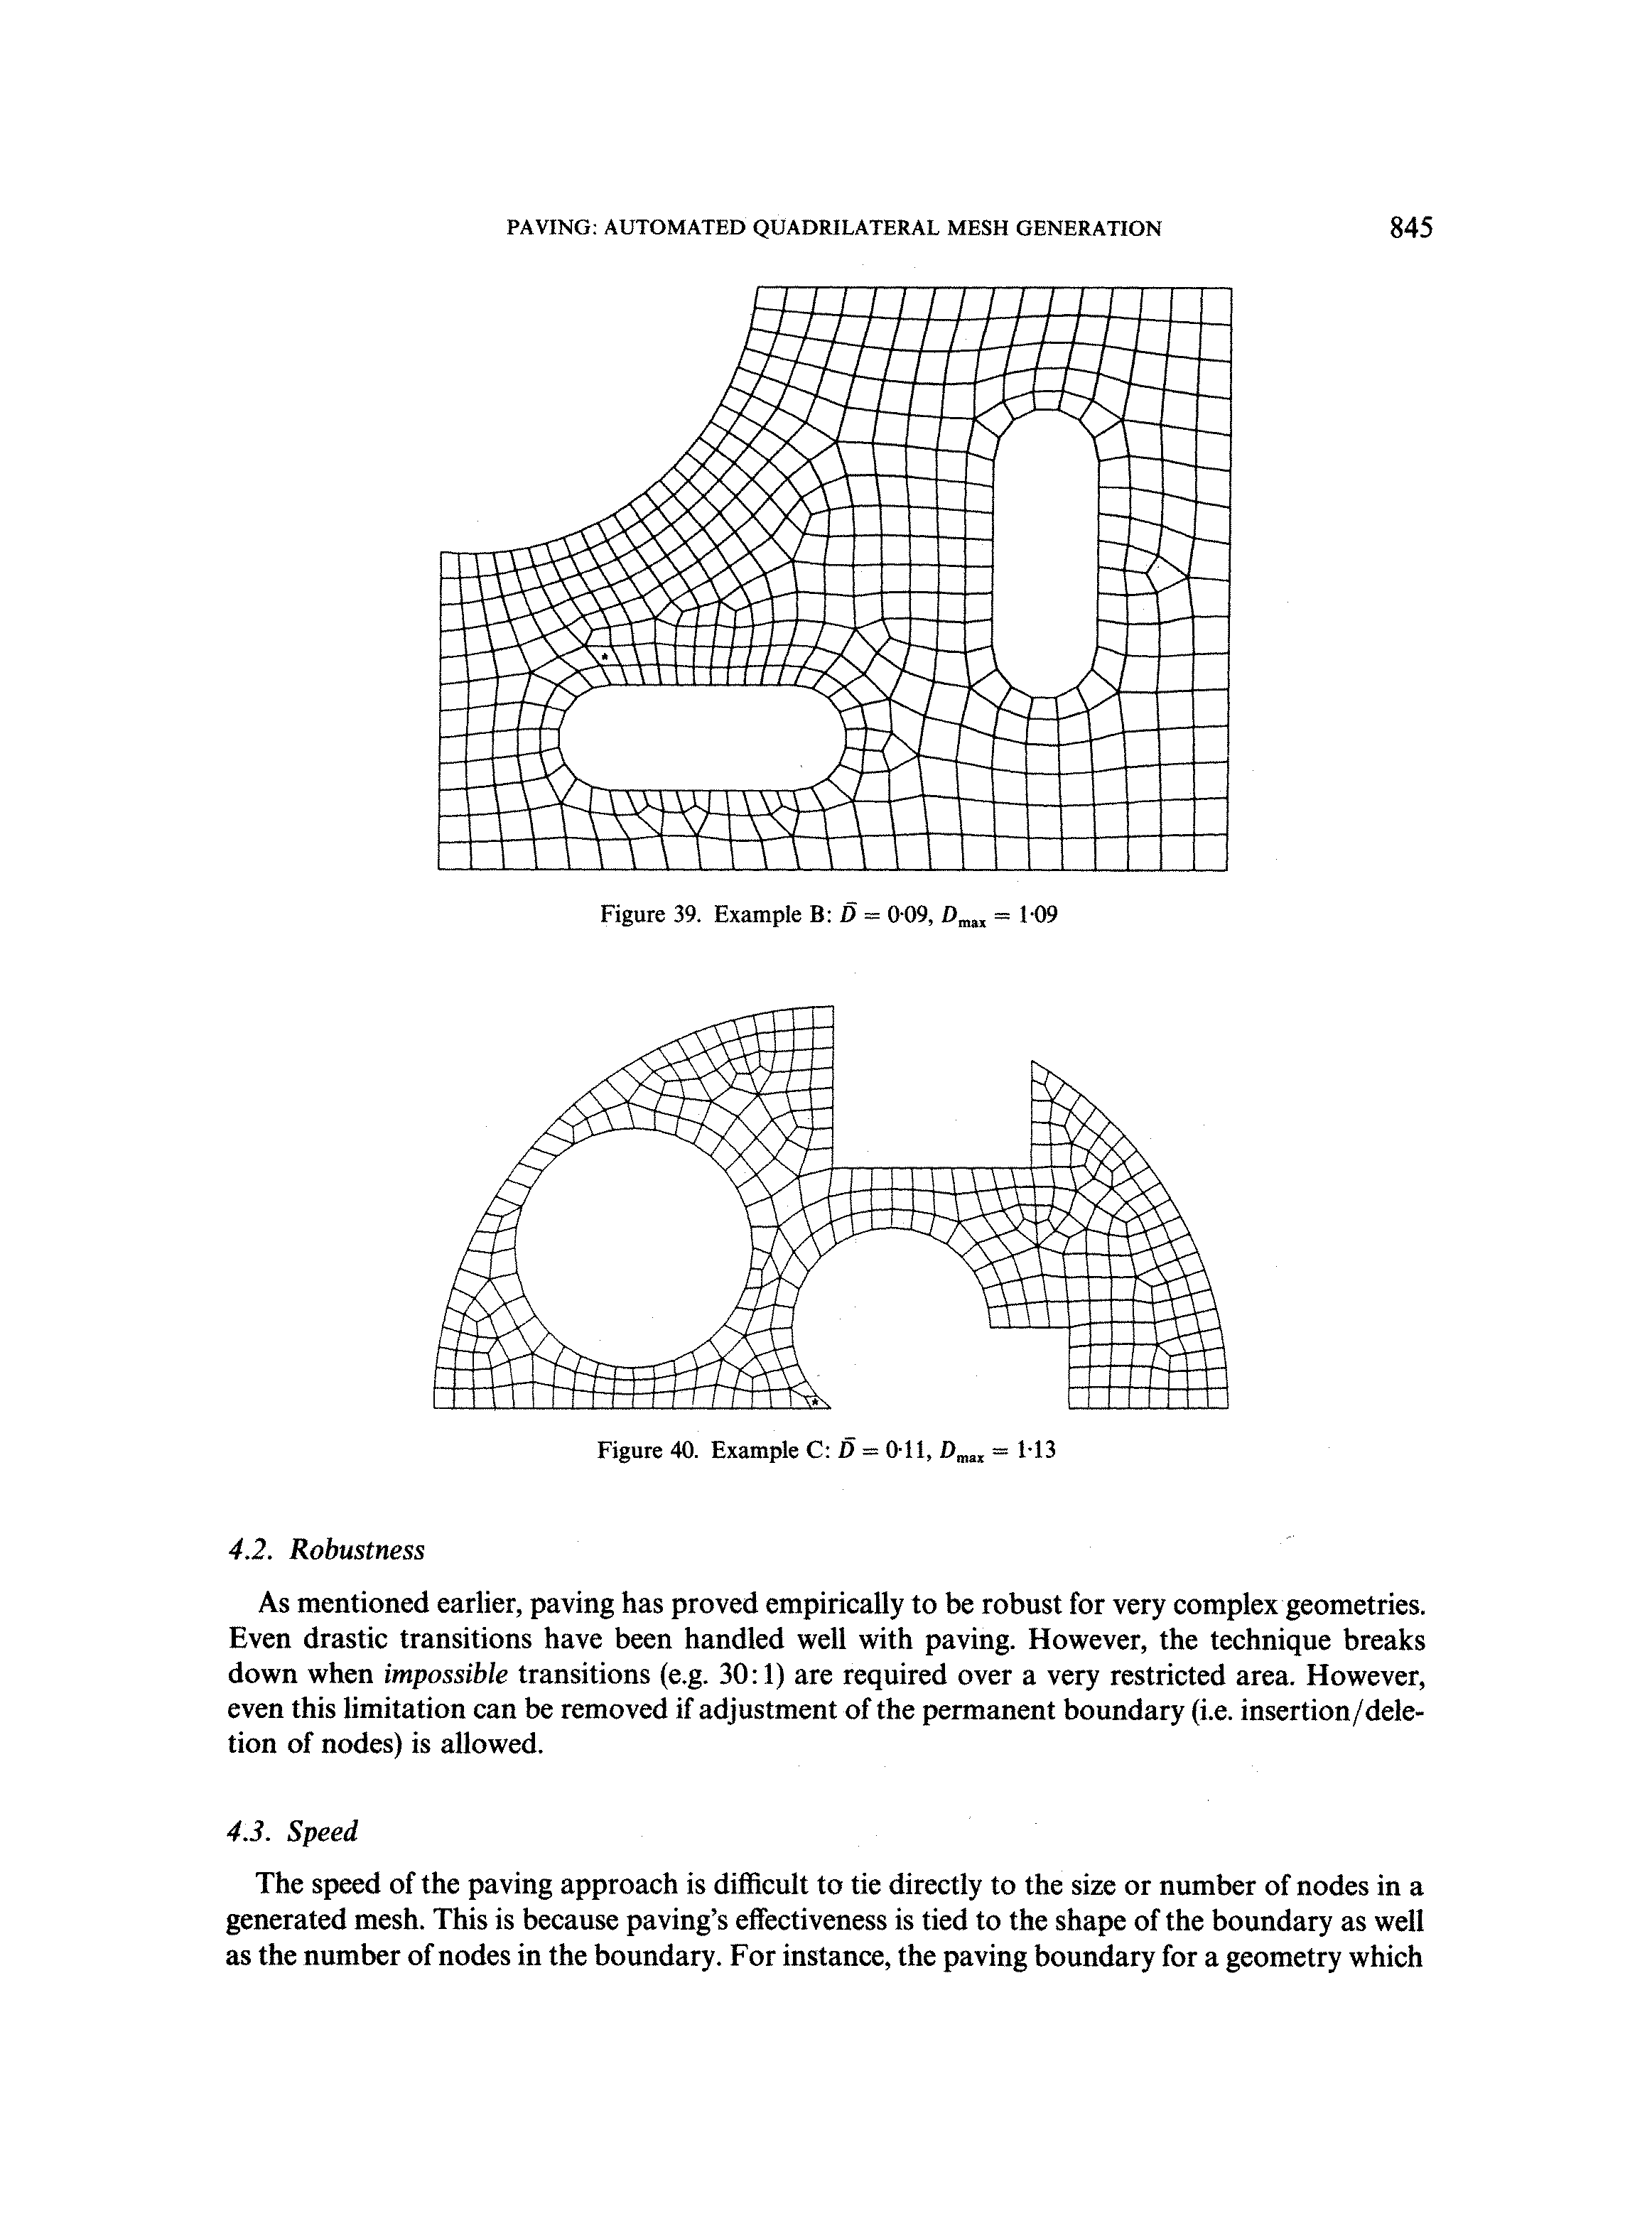
\includegraphics[trim={0 65.5cm 0 14cm },clip,width=\linewidth]{img/intro/lit/quadMesh.png}
	\caption{A non-simplical quad mesh generated with paving methodology \cite{blacker1991paving}.}
	\label{fig-quadMesh}
\end{figure}

Even though non-simplical mesh elements have been favored for a variety of scenrarios in mesh generation, and especially while generating highly-stretched elements, they have their cons. It is significantly difficult to generate an automatic mesh generation strategy which creates non-simplicial mesh conforming to complex surface and 3D geometrical configurations. Manual input is usually required to mesh such geometries. In these situations, simplical mesh elements are quite useful in dealing with the complexity in the geometry. Hence, a hybrid mesh containing both simplical and non-simplical mesh elements is a reasonable choice for mesh generation. We would revisit this in section \ref{sec-motivation} where we reason about choosing a hybrid scheme to mesh the surface.

\section{Boundary Layer Meshes}
\label{sec-boundaryLayerMesh}

With the advent of several unstructured mesh generation techniques (cite them), a broader selection of geometries could be dealt with. This immensely increased the scope of CFD solvers and pushed the limits of numerical methods in terms of accuracy and speed. However, a different approach was needed for the parts of the mesh in which viscous forces were more dominant as compared to the inertial forces. In other words, at the location of the viscous boundary layer, the gradient of physical measures like velocity is several magnitudes higher in one direction as compared to its orthogonal direction. A mesh generation technique which would help in resolving such strong gradients of the velocity in the boundary layer was required. For example, consider a flow over a flat plate as shown in Figure \ref{fig-boundaryLayer}. The velocity of the fluid at the surface of the plate is zero. However, the velocity becomes freestream velocity $u_0$ very near to the surface. The thickness of this layer of fluid, where the freestream velocit	y goes from a value of zero to a value of around 0.95 times the freestream velocity is called as the boundary layer thickness $\delta$. It is also called the viscous boundary layer as the viscous effects are dominant in this layer.

\begin{figure}
  \centering	
  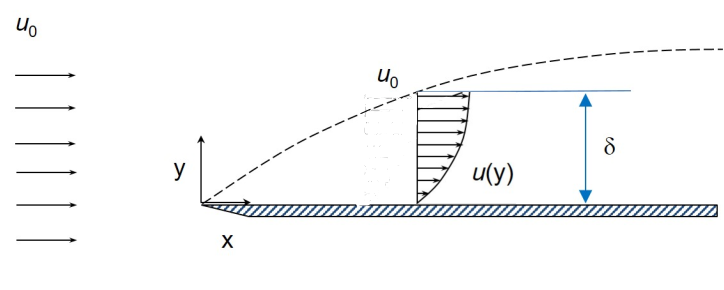
\includegraphics[width=0.8\linewidth]{img/intro/boundaryLayer.jpg}
  \caption{Fluid flow over a flat plate.}
  \label{fig-boundaryLayer}
\end{figure}

\section{Anisotropic Meshing}

The need to resolve the steep gradients at the boundary layer of the fluid flow gave rise to a type of mesh development strategy called anisotropic meshing. An anisotropic mesh is simply a mesh which has highly stretched elements. In other words, the aspect ratio of the elements for an anisotropic mesh would be really high. Such a packing of the cell elements is required to provide a large number of Degree Of Freedom (DOF) along the direction of steep gradients of physical quantities such as velocity. Traditionally generated isotropic meshes are incapable of resolving such steep gradients \cite{frey2005anisotropic}. 

\begin{figure}
	\centering
	\begin{subfigure}{0.5\linewidth}
	  \centering
	  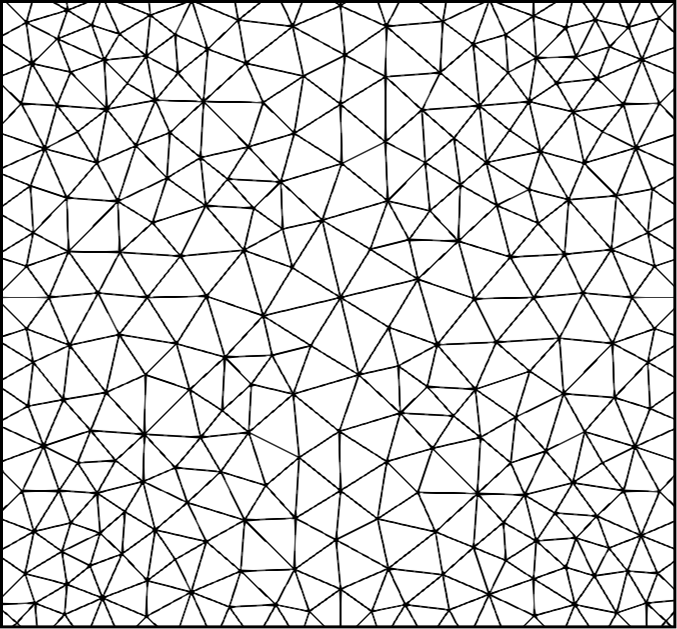
\includegraphics[width=0.9\linewidth]{img/intro/isotropic.png}
	  \caption{Isotropic mesh}
	  \label{fig-isotropic}
	\end{subfigure}%
	\begin{subfigure}{0.5\linewidth}
		\centering
		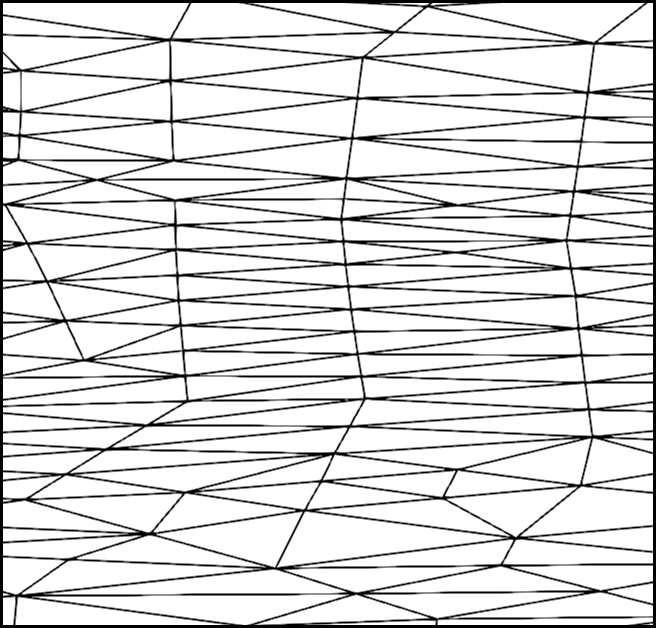
\includegraphics[width=0.88\linewidth]{img/intro/anisotropic.png}
		\caption{Anisotropic Mesh}
		\label{fig-anisotropic}
	\end{subfigure}
	\caption{Isotropic and Anisotropic Mesh Fragments}
	\label{fig-isotropic-anisotropic}
\end{figure}

Figure \ref{fig-isotropic} shows an isotropic mesh. The mesh elements have almost equal edge lengths. Here, the mesh elements are triangles and resemble equilateral triangles for most parts of the mesh. Given a point in the mesh, all the directions are the same and there isn't any bias towards a particular direction. For an isotropic physical process, such a mesh will serve the purpose and resolve gradients in all directions given the resolution of the mesh is appropriately chosen. However, if the physical process to be simulated is highly anisotropic, such as the velocity distribution along the boundary layer of the flat plate, as discussed in section \ref{sec-boundaryLayerMesh}, such a mesh will fail to resolve the steep velocity gradients. It would have to be refined to get the required refinement at the boundary, increasing the total number of DOFs in the mesh by a polynomial factor. Hence, a more reasonable mesh generation strategy is needed.

Figure \ref{fig-anisotropic} shows an anisotropic mesh. The triangular elements of the mesh are highly streched, with one edge being considerably shorter than the other two. The number of DOFs is distributed over the domain in a fashion so as to have the majority of the DOFs along the steep gradients of the physical quantities to be simulated. Hence, cell alignment with the solution to capture anisotropic flow features is possible with such a mesh.

\begin{figure}
	\centering
	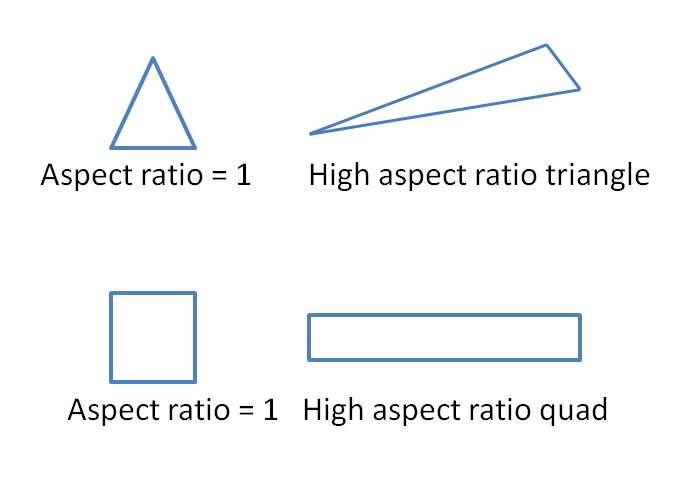
\includegraphics[width=0.8\linewidth]{img/intro/aspectRatio.png}
	\caption{Illustration of different aspect ratio triangular and quadrilateral elements.}
\end{figure}

\subsection{Brief Literature Review - Anisotropic Meshing}

Several techniques have been developed to generate meshes in two dimensions with some sort of anisotropy. Some of these techniques have also been generalized to surfaces. However, isotropically-meshed surfaces with a smooth element-size variation are generally easier to mesh than anisotropically-meshed surfaces with strong size variations \cite{TU2013219}. Many techniques developed in 2D have been generalized to 3D while some new methodologies have been deviced for volume meshing. We go over some of these methods briefly.

\subsubsection{2D and Surfaces}

Most of the initial attempts at generating stretched element meshes in two dimensions used a Delaunay mesh and a locally mapped space to get the required level of anisotropy  \cite{mavriplis1990adaptive}. A mesh generated by such a method is shown in Figure \ref{fig-mavri}. Some techniques used an approach of using a locally structured or semi structured mesh for the regions requiring high anisotropy  \cite{nakahashi1987fdm}.

\begin{figure*}
\centering
\begin{minipage}[b]{.4\textwidth}
	\centering
	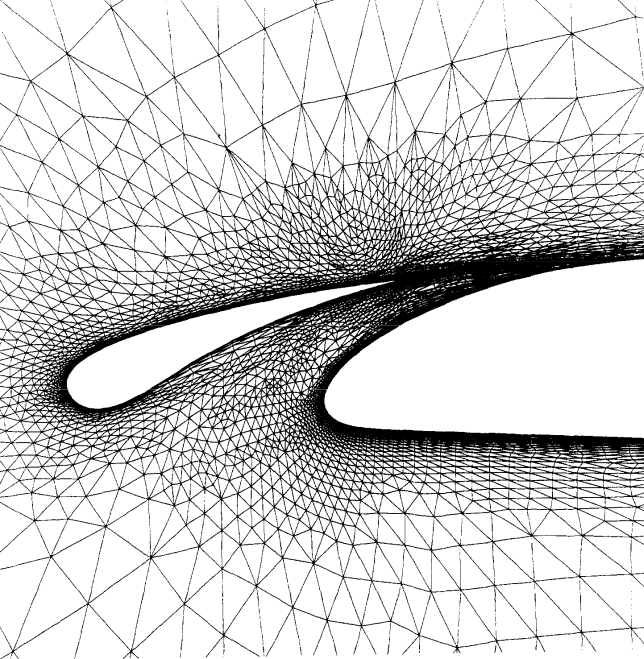
\includegraphics[width=\linewidth]{img/intro/lit/mavri.png}
	\caption{Illustration of adaptively refined mesh for the two-element airfoil configuration near the gap region \cite{mavriplis1990adaptive}.}
	\label{fig-mavri}
\end{minipage}\hfill
\begin{minipage}[b]{.55\textwidth}
	\centering
	\begin{subfigure}{\linewidth}
	\centering
	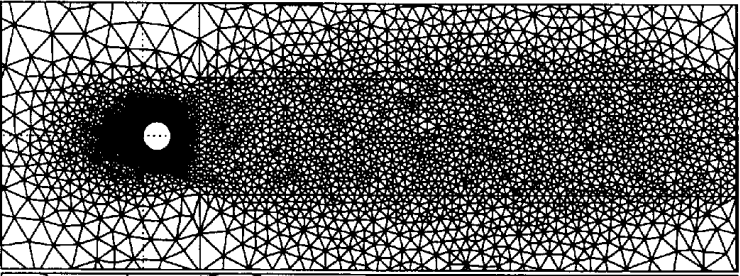
\includegraphics[width=\linewidth]{img/intro/lit/castroInitial.png}
	\caption{}
	\label{fig-castroInitial}
	\end{subfigure}
	\begin{subfigure}{\linewidth}
		\centering
		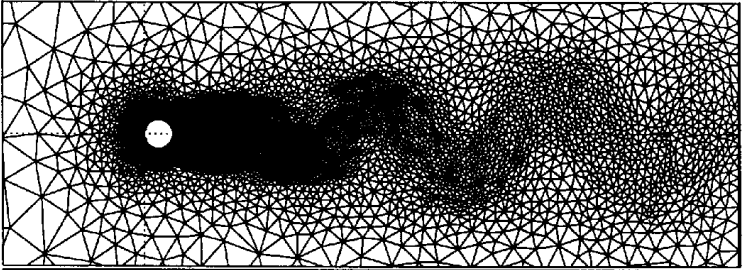
\includegraphics[width=\linewidth]{img/intro/lit/castro.png}
		\caption{}
	\label{fig-castro}
	\end{subfigure}
	\caption{Initial mesh (a) and adaptively generated anisotropic mesh (b) using solution metric evaluation	\cite{castro1997anisotropic}.}
\end{minipage}
\end{figure*}

Many attempts at generating anisotropic meshes come under the category of metric adaptation of the mesh. These techniques generally used a Delaunay type initial mesh and refined it anisotropically using a solution metric. Shimada \etal provided an automated method to obtain anisotropic triangulation of a parametric surface. Given a domain geometry and a tensor field that specifies desired anisotropic node-spacing, a proximity-based interacting force field is defined and the force balance configuration is dynamically simulated \cite{shimada1997anisotropic}. Castro \etal applied mesh adaptation technique to generate anisotropic meshes, to compressible viscous flows for a wide range of Reynolds and Mach numbers \cite{castro1997anisotropic}. An illustration of this method can be seen in Figure \ref{fig-castro}. 

Kunert \etal showed an anisotropic mesh generation algorithm that refines the mesh anisotropically by calculating the local error estimate on the initial mesh \cite{kunert2002toward}. This algorithm was presented for both two dimensional and three dimensional meshes. Another mesh adaptation technique by Li \etal tried to align the mesh to a calculated metric tensor from the physics of the problem \cite{li2010anisotropic}. Figure \ref{fig-anisotropicMeshAdaptation} shows one such mesh.

\begin{figure*}
\centering
\begin{minipage}[b]{.44\textwidth}
	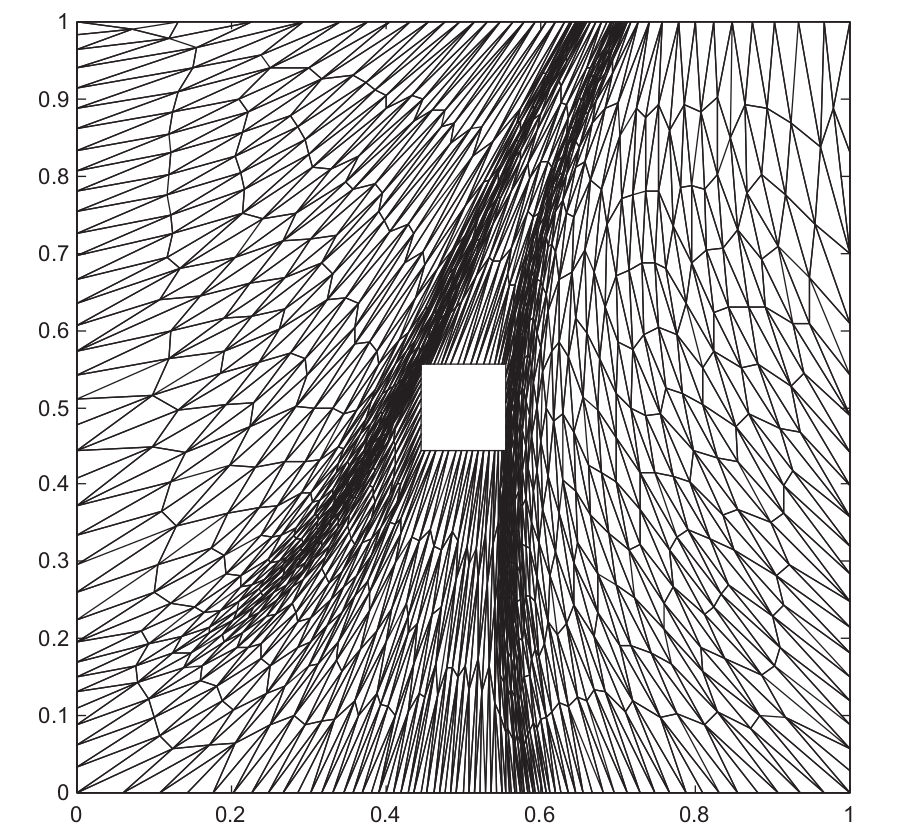
\includegraphics[width=\linewidth]{img/intro/lit/anisotropicMeshAdaptation.png}
	\caption{Anisotropic mesh generated by aligning the mesh elements to a metric calculated from an isotropic mesh solution \cite{li2010anisotropic}.}
	\label{fig-anisotropicMeshAdaptation}
\end{minipage}\hfill
\begin{minipage}[b]{.44\textwidth}
	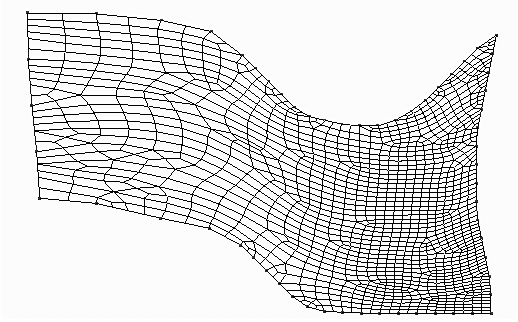
\includegraphics[width=\linewidth]{img/intro/lit/anisotropicQuadMesh.png}
	\caption{Anisotropic quadrilateral mesh generated with an input triangulation and solution contours \cite{viswanath2000quadrilateral}.}
	\label{fig-anisotropicQuadMesh}
\end{minipage}
\end{figure*}

A family of anisotropic mesh generation techniques fall under the Advancing Layer category. A method introduced by Pirzadeh produced unstructured triangular/tetrahedral grids with high-aspect-ratio cells using the advancing layer or the grid-marching strategy \cite{pirzadeh1994unstructured}. Another method which used the advancing layer strategy, with several mesh collision checks, was introduced by Lohner \cite{lohner1993matching}. Here, the mesh was produced by inflating the boundary curves in the direction of surface normals. Special care was taken while dealing with the concave corners of the mesh so as to avoid mesh element collisions.

While the majority of anisotropic mesh generation strategies focused on simplicial mesh elements, there have been some works which generate all quadrilateral (quad) surface meshes. A method by Lee \etal showed an anisotropic quadrilateral mesh generation scheme which generates a background triangular mesh and then proceeding with a cell merging procedure in the parametric space to produce the desired mesh \cite{lee2003new}. A different kind of method was adopted by Viswanath \etal to generate quadrilateral meshes with anisotropy and directional control \cite{viswanath2000quadrilateral}. A 2D geometric domain and desired level of anisotropy - as a metric tensor over the domain - specifying mesh sizing in two independent directions is taken as an input. Thereby node locations are calculated by closely packing recctangles in accordance with the inputs. An example mesh generated with this strategy is shown in Figure \ref{fig-anisotropicQuadMesh}.

\subsubsection{3D}

Several methods which generate 2D meshes can be extended to 3D \cite{lohner1993matching, nakahashi1987fdm,castro1997anisotropic}.

The method used by Shimada and Yamada in two dimensions has also been extended to three dimensions to generate anisotropic tetrahedral meshes. Given an arbitrary input anisotropy function, the algorithm generates high quality anisotropic tetrahedral mesh that conforms to the input geometry \cite{yamakawa2000high}.

\begin{figure}
	\centering
	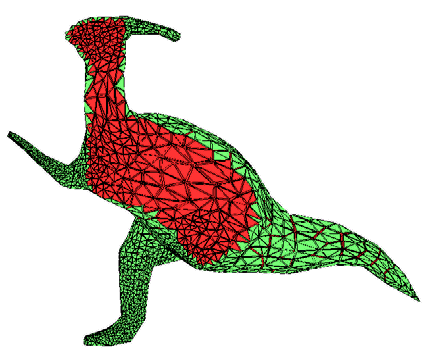
\includegraphics[width=0.5\linewidth]{img/intro/lit/highQualityTetMesh.png}
	\caption{Anisotropic Tetrahedral Mesh generated using ellipsoidal bubble packing methodology  \cite{yamakawa2000high}}
	\label{fig-anisotropicTetMesh}
\end{figure}

In another work, a metric-orthogonal anisotropic mesh is generated by aligning the mesh to a metric, mesh elements are also aligned with teh eigenvectors \cite{loseille20093d}. The quality of the input metric strongly affects the output mesh.

\section{Motivation}
\label{sec-motivation}

The methods mentioned above generate good quality anisotropic meshes. However, they have some drawbacks. Firstly, almost all of the methodologies which produce anisotropic meshes generate simplicial mesh elements. These simplicial meshes have an advantage of good flexibility in descretizing the domain, especially if it contains complex features. However, the vertex connectivity of simplicial mesh elements is high. The number of edges in a tetrahedral mesh is about seven times the number of vertices. On the other hand, in a hexahedral mesh, the number of edges is only about three times the number of vertices (asymptotically). The cost of vertex-based discretization is directly proportional to the number of edges in a mesh. Hence, non-simplicial meshes are substantially more efficient than simplicial meshes for a given number of unknowns or grid points. Also, regular arrays of nonsimplicial elements may also enhance accuracy, owing to a local cancellation of truncation errors that may not occur on groups of nonsimilar simplicial elements \cite{mavriplis1997unstructured}.

Non-simplicial quadrilateral elements have been preferred over triangles in highly stretched two-dimensional grids due to their lower connectivity \cite{aftosmis1994accuracy}. The advantages of non-simplicial mesh elements have resulted in fully non-simplicial mesh generation techniques \cite{blacker1991paving, zhu1991new}.

\section{Surface Meshing}
\section{Outline}
